\chapter{深度優先搜索}


\section{Palindrome Partitioning} %%%%%%%%%%%%%%%%%%%%%%%%%%%%%%
\label{sec:palindrome-partitioning}


\subsubsection{描述}
Given a string s, partition s such that every substring of the partition is a palindrome.

Return all possible palindrome partitioning of s.

For example, given \code{s = "aab"},
Return
\begin{Code}
  [
    ["aa","b"],
    ["a","a","b"]
  ]
\end{Code}


\subsubsection{分析}
在每一步都可以判斷中間結果是否為合法結果,用回溯法。

一個長度為n的字符串,有$n-1$個地方可以砍斷,每個地方可斷可不斷,因此複雜度為$O(2^{n-1})$


\subsubsection{深搜1}
\begin{Code}
//LeetCode, Palindrome Partitioning
// 時間複雜度O(2^n),空間複雜度O(n)
class Solution {
public:
    vector<vector<string>> partition(string s) {
        vector<vector<string>> result;
        vector<string> path;  // 一個partition方案
        dfs(s, path, result, 0, 1);
        return result;
    }

    // prev 表示前一個隔板, start 表示當前隔板
    void dfs(string &s, vector<string>& path,
            vector<vector<string>> &result, size_t prev, size_t start) {
        if (start == s.size()) { // 最後一個隔板
            if (isPalindrome(s, prev, start - 1)) { // 必須使用
                path.push_back(s.substr(prev, start - prev));
                result.push_back(path);
                path.pop_back();
            }
            return;
        }
        // 不斷開
        dfs(s, path, result, prev, start + 1);
        // 如果[prev, start-1] 是迴文,則可以斷開,也可以不斷開(上一行已經做了)
        if (isPalindrome(s, prev, start - 1)) {
            // 斷開
            path.push_back(s.substr(prev, start - prev));
            dfs(s, path, result, start, start + 1);
            path.pop_back();
        }
    }

    bool isPalindrome(const string &s, int start, int end) {
        while (start < end && s[start] == s[end]) {
            ++start;
            --end;
        }
        return start >= end;
    }
};
\end{Code}

\subsubsection{深搜2}
另一種寫法,更加簡潔。這種寫法也在 Combination Sum, Combination Sum II 中出現過。
\begin{Code}
//LeetCode, Palindrome Partitioning
// 時間複雜度O(2^n),空間複雜度O(n)
class Solution {
public:
    vector<vector<string>> partition(string s) {
        vector<vector<string>> result;
        vector<string> path;  // 一個partition方案
        DFS(s, path, result, 0);
        return result;
    }
    // 搜索必須以s[start]開頭的partition方案
    void DFS(string &s, vector<string>& path,
            vector<vector<string>> &result, int start) {
        if (start == s.size()) {
            result.push_back(path);
            return;
        }
        for (int i = start; i < s.size(); i++) {
            if (isPalindrome(s, start, i)) { // 從i位置砍一刀
                path.push_back(s.substr(start, i - start + 1));
                DFS(s, path, result, i + 1);  // 繼續往下砍
                path.pop_back(); // 撤銷上上行
            }
        }
    }
    bool isPalindrome(const string &s, int start, int end) {
        while (start < end && s[start] == s[end]) {
            ++start;
            --end;
        }
        return start >= end;
    }
};
\end{Code}


\subsubsection{動規}
\begin{Code}
// LeetCode, Palindrome Partitioning
// 動規,時間複雜度O(n^2),空間複雜度O(1)
class Solution {
public:
    vector<vector<string> > partition(string s) {
        const int n = s.size();
        bool p[n][n]; // whether s[i,j] is palindrome
        fill_n(&p[0][0], n * n, false);
        for (int i = n - 1; i >= 0; --i)
            for (int j = i; j < n; ++j)
                p[i][j] = s[i] == s[j] && ((j - i < 2) || p[i + 1][j - 1]);

        vector<vector<string> > sub_palins[n]; // sub palindromes of s[0,i]
        for (int i = n - 1; i >= 0; --i) {
            for (int j = i; j < n; ++j)
                if (p[i][j]) {
                    const string palindrome = s.substr(i, j - i + 1);
                    if (j + 1 < n) {
                        for (auto v : sub_palins[j + 1]) {
                            v.insert(v.begin(), palindrome);
                            sub_palins[i].push_back(v);
                        }
                    } else {
                        sub_palins[i].push_back(vector<string> { palindrome });
                    }
                }
        }
        return sub_palins[0];
    }
};
\end{Code}


\subsubsection{相關題目}

\begindot
\item Palindrome Partitioning II,見 \S \ref{sec:palindrome-partitioning-ii}
\myenddot


\section{Unique Paths} %%%%%%%%%%%%%%%%%%%%%%%%%%%%%%
\label{sec:unique-paths}


\subsubsection{描述}
A robot is located at the top-left corner of a $m \times n$ grid (marked 'Start' in the diagram below).

The robot can only move either down or right at any point in time. The robot is trying to reach the bottom-right corner of the grid (marked 'Finish' in the diagram below).

How many possible unique paths are there?

\begin{center}
\includegraphics[width=200pt]{robot-maze.png}\\
\figcaption{Above is a $3 \times 7$ grid. How many possible unique paths are there?}\label{fig:unique-paths}
\end{center}

\textbf{Note}: $m$ and $n$ will be at most 100.


\subsection{深搜}
深搜,小集合可以過,大集合會超時

\subsubsection{代碼}
\begin{Code}
// LeetCode, Unique Paths
// 深搜,小集合可以過,大集合會超時
// 時間複雜度O(n^4),空間複雜度O(n)
class Solution {
public:
    int uniquePaths(int m, int n) {
        if (m < 1 || n < 1) return 0; // 終止條件

        if (m == 1 && n == 1) return 1; // 收斂條件

        return uniquePaths(m - 1, n) + uniquePaths(m, n - 1);
    }
};
\end{Code}


\subsection{備忘錄法}
給前面的深搜,加個緩存,就可以過大集合了。即備忘錄法。

\subsubsection{代碼}
\begin{Code}
// LeetCode, Unique Paths
// 深搜 + 緩存,即備忘錄法
// 時間複雜度O(n^2),空間複雜度O(n^2)
class Solution {
public:
    int uniquePaths(int m, int n) {
        // f[x][y] 表示 從(0,0)到(x,y)的路徑條數
        f = vector<vector<int> >(m, vector<int>(n, 0));
        f[0][0] = 1;
        return dfs(m - 1, n - 1);
    }
private:
    vector<vector<int> > f;  // 緩存

    int dfs(int x, int y) {
        if (x < 0 || y < 0) return 0; // 數據非法,終止條件

        if (x == 0 && y == 0) return f[0][0]; // 回到起點,收斂條件

        if (f[x][y] > 0) {
            return f[x][y];
        } else {
            return f[x][y] = dfs(x - 1, y) +  dfs(x, y - 1);
        }
    }
};
\end{Code}


\subsection{動規}
既然可以用備忘錄法自頂向下解決,也一定可以用動規自底向上解決。

設狀態為\fn{f[i][j]},表示從起點$(1,1)$到達$(i,j)$的路線條數,則狀態轉移方程為:
\begin{Code}
f[i][j]=f[i-1][j]+f[i][j-1]
\end{Code}


\subsubsection{代碼}
\begin{Code}
// LeetCode, Unique Paths
// 動規,滾動數組
// 時間複雜度O(n^2),空間複雜度O(n)
class Solution {
public:
    int uniquePaths(int m, int n) {
        vector<int> f(n, 0);
        f[0] = 1;
        for (int i = 0; i < m; i++) {
            for (int j = 1; j < n; j++) {
                // 左邊的f[j],表示更新後的f[j],與公式中的f[i][j]對應
                // 右邊的f[j],表示老的f[j],與公式中的f[i-1][j]對應
                f[j] = f[j] + f[j - 1];
            }
        }
        return f[n - 1];
    }
};
\end{Code}


\subsection{數學公式}
一個$m$行,$n$列的矩陣,機器人從左上走到右下總共需要的步數是$m+n-2$,其中向下走的步數是$m-1$,因此問題變成了在$m+n-2$個操作中,選擇$m–1$個時間點向下走,選擇方式有多少種。即 $C_{m+n-2}^{m-1}$ 。

\subsubsection{代碼}
\begin{Code}
// LeetCode, Unique Paths
// 數學公式
class Solution {
public:
    typedef long long int64_t;
    // 求階乘, n!/(start-1)!,即 n*(n-1)...start,要求 n >= 1
    static int64_t factor(int n, int start = 1) {
        int64_t  ret = 1;
        for(int i = start; i <= n; ++i)
            ret *= i;
        return ret;
    }
    // 求組合數 C_n^k
    static int64_t combination(int n, int k) {
        // 常數優化
        if (k == 0) return 1;
        if (k == 1) return n;

        int64_t ret = factor(n, k+1);
        ret /= factor(n - k);
        return ret;
    }

    int uniquePaths(int m, int n) {
        // max 可以防止n和k差距過大,從而防止combination()溢出
        return combination(m+n-2, max(m-1, n-1));
    }
};
\end{Code}


\subsubsection{相關題目}
\begindot
\item Unique Paths II,見 \S \ref{sec:unique-paths-ii}
\item Minimum Path Sum, 見 \S \ref{sec:minimum-path-sum}
\myenddot


\section{Unique Paths II} %%%%%%%%%%%%%%%%%%%%%%%%%%%%%%
\label{sec:unique-paths-ii}


\subsubsection{描述}
Follow up for "Unique Paths":

Now consider if some obstacles are added to the grids. How many unique paths would there be?

An obstacle and empty space is marked as 1 and 0 respectively in the grid.

For example,

There is one obstacle in the middle of a $3 \times 3$ grid as illustrated below.
\begin{Code}
[
  [0,0,0],
  [0,1,0],
  [0,0,0]
]
\end{Code}

The total number of unique paths is 2.

Note: $m$ and $n$ will be at most 100.


\subsection{備忘錄法}
在上一題的基礎上改一下即可。相比動規,簡單得多。

\subsubsection{代碼}
\begin{Code}
// LeetCode, Unique Paths II
// 深搜 + 緩存,即備忘錄法
class Solution {
public:
    int uniquePathsWithObstacles(const vector<vector<int> >& obstacleGrid) {
        const int m = obstacleGrid.size();
        const int n = obstacleGrid[0].size();
        if (obstacleGrid[0][0] || obstacleGrid[m - 1][n - 1]) return 0;

        f = vector<vector<int> >(m, vector<int>(n, 0));
        f[0][0] = obstacleGrid[0][0] ? 0 : 1;
        return dfs(obstacleGrid, m - 1, n - 1);
    }
private:
    vector<vector<int> > f;  // 緩存

    // @return 從 (0, 0) 到 (x, y) 的路徑總數
    int dfs(const vector<vector<int> >& obstacleGrid,
            int x, int y) {
        if (x < 0 || y < 0) return 0; // 數據非法,終止條件

        // (x,y)是障礙
        if (obstacleGrid[x][y]) return 0;

        if (x == 0 and y == 0) return f[0][0]; // 回到起點,收斂條件

        if (f[x][y] > 0) {
            return f[x][y];
        } else {
            return f[x][y] = dfs(obstacleGrid, x - 1, y) + 
                dfs(obstacleGrid, x, y - 1);
        }
    }
};
\end{Code}


\subsection{動規}
與上一題類似,但要特別注意第一列的障礙。在上一題中,第一列全部是1,但是在這一題中不同,第一列如果某一行有障礙物,那麼後面的行全為0。


\subsubsection{代碼}
\begin{Code}
// LeetCode, Unique Paths II
// 動規,滾動數組
// 時間複雜度O(n^2),空間複雜度O(n)
class Solution {
public:
    int uniquePathsWithObstacles(vector<vector<int> > &obstacleGrid) {
        const int m = obstacleGrid.size();
        const int n = obstacleGrid[0].size();
        if (obstacleGrid[0][0] || obstacleGrid[m-1][n-1]) return 0;

        vector<int> f(n, 0);
        f[0] = obstacleGrid[0][0] ? 0 : 1;

        for (int i = 0; i < m; i++) {
            f[0] = f[0] == 0 ? 0 : (obstacleGrid[i][0] ? 0 : 1);
            for (int j = 1; j < n; j++)
                f[j] = obstacleGrid[i][j] ? 0 : (f[j] + f[j - 1]);
        }

        return f[n - 1];
    }
};
\end{Code}


\subsubsection{相關題目}
\begindot
\item Unique Paths,見 \S \ref{sec:unique-paths}
\item Minimum Path Sum, 見 \S \ref{sec:minimum-path-sum}
\myenddot


\section{N-Queens} %%%%%%%%%%%%%%%%%%%%%%%%%%%%%%
\label{sec:n-queens}


\subsubsection{描述}
The \emph{n-queens puzzle} is the problem of placing n queens on an $n \times n$ chessboard such that no two queens attack each other.

\begin{center}
\includegraphics{8-queens.png}\\
\figcaption{Eight Queens}\label{fig:8-queens}
\end{center}

Given an integer $n$, return all distinct solutions to the n-queens puzzle.

Each solution contains a distinct board configuration of the n-queens' placement, where \fn{'Q'} and \fn{'.'} both indicate a queen and an empty space respectively.

For example,
There exist two distinct solutions to the 4-queens puzzle:
\begin{Code}
[
 [".Q..",  // Solution 1
  "...Q",
  "Q...",
  "..Q."],

 ["..Q.",  // Solution 2
  "Q...",
  "...Q",
  ".Q.."]
]
\end{Code}


\subsubsection{分析}

經典的深搜題。

設置一個數組 \fn{vector<int> C(n, 0)}, \fn{C[i]} 表示第i行皇后所在的列編號,即在位置 (i, C[i]) 上放了一個皇后,這樣用一個一維數組,就能記錄整個棋盤。


\subsubsection{代碼1}
\begin{Code}
// LeetCode, N-Queens
// 深搜+剪枝
// 時間複雜度O(n!*n),空間複雜度O(n)
class Solution {
public:
    vector<vector<string> > solveNQueens(int n) {
        vector<vector<string> > result;
        vector<int> C(n, -1);  // C[i]表示第i行皇后所在的列編號
        dfs(C, result, 0);
        return result;
    }
private:
    void dfs(vector<int> &C, vector<vector<string> > &result, int row) {
        const int N = C.size();
        if (row == N) { // 終止條件,也是收斂條件,意味着找到了一個可行解
            vector<string> solution;
            for (int i = 0; i < N; ++i) {
                string s(N, '.');
                for (int j = 0; j < N; ++j) {
                    if (j == C[i]) s[j] = 'Q';
                }
                solution.push_back(s);
            }
            result.push_back(solution);
            return;
        }

        for (int j = 0; j < N; ++j) {  // 擴展狀態,一列一列的試
            const bool ok = isValid(C, row, j);
            if (!ok) continue;  // 剪枝,如果非法,繼續嘗試下一列
            // 執行擴展動作
            C[row] = j;
            dfs(C, result, row + 1);
            // 撤銷動作
            // C[row] = -1;
        }
    }
    
    /**
     * 能否在 (row, col) 位置放一個皇后.
     *
     * @param C 棋局
     * @param row 當前正在處理的行,前面的行都已經放了皇后了
     * @param col 當前列
     * @return 能否放一個皇后
     */
    bool isValid(const vector<int> &C, int row, int col) {
        for (int i = 0; i < row; ++i) {
            // 在同一列
            if (C[i] == col) return false;
            // 在同一對角線上
            if (abs(i - row) == abs(C[i] - col)) return false;
        }
        return true;
    }
};
\end{Code}


\subsubsection{代碼2}
\begin{Code}
// LeetCode, N-Queens
// 深搜+剪枝
// 時間複雜度O(n!),空間複雜度O(n)
class Solution {
public:
    vector<vector<string> > solveNQueens(int n) {
        this->columns = vector<bool>(n, false);
        this->main_diag = vector<bool>(2 * n - 1, false);
        this->anti_diag = vector<bool>(2 * n - 1, false);

        vector<vector<string> > result;
        vector<int> C(n, -1);  // C[i]表示第i行皇后所在的列編號
        dfs(C, result, 0);
        return result;
    }
private:
    // 這三個變量用於剪枝
    vector<bool> columns;  // 表示已經放置的皇后佔據了哪些列
    vector<bool> main_diag;  // 佔據了哪些主對角線
    vector<bool> anti_diag;  // 佔據了哪些副對角線

    void dfs(vector<int> &C, vector<vector<string> > &result, int row) {
        const int N = C.size();
        if (row == N) { // 終止條件,也是收斂條件,意味着找到了一個可行解
            vector<string> solution;
            for (int i = 0; i < N; ++i) {
                string s(N, '.');
                for (int j = 0; j < N; ++j) {
                    if (j == C[i]) s[j] = 'Q';
                }
                solution.push_back(s);
            }
            result.push_back(solution);
            return;
        }

        for (int j = 0; j < N; ++j) {  // 擴展狀態,一列一列的試
            const bool ok = !columns[j] && !main_diag[row - j + N - 1]  &&
                    !anti_diag[row + j];
            if (!ok) continue;  // 剪枝,如果非法,繼續嘗試下一列
            // 執行擴展動作
            C[row] = j;
            columns[j] = main_diag[row - j + N - 1] = anti_diag[row + j] = true;
            dfs(C, result, row + 1);
            // 撤銷動作
            // C[row] = -1;
            columns[j] = main_diag[row - j + N - 1] = anti_diag[row + j] = false;
        }
    }
};
\end{Code}


\subsubsection{相關題目}
\begindot
\item N-Queens II,見 \S \ref{sec:n-queens-ii}
\myenddot


\section{N-Queens II} %%%%%%%%%%%%%%%%%%%%%%%%%%%%%%
\label{sec:n-queens-ii}


\subsubsection{描述}
Follow up for N-Queens problem.

Now, instead outputting board configurations, return the total number of distinct solutions.


\subsubsection{分析}
只需要輸出解的個數,不需要輸出所有解,代碼要比上一題簡化很多。設一個全局計數器,每找到一個解就增1。


\subsubsection{代碼1}
\begin{Code}
// LeetCode, N-Queens II
// 深搜+剪枝
// 時間複雜度O(n!*n),空間複雜度O(n)
class Solution {
public:
    int totalNQueens(int n) {
        this->count = 0;

        vector<int> C(n, 0);  // C[i]表示第i行皇后所在的列編號
        dfs(C, 0);
        return this->count;
    }
private:
    int count; // 解的個數

    void dfs(vector<int> &C, int row) {
        const int N = C.size();
        if (row == N) { // 終止條件,也是收斂條件,意味着找到了一個可行解
            ++this->count;
            return;
        }

        for (int j = 0; j < N; ++j) {  // 擴展狀態,一列一列的試
            const bool ok = isValid(C, row, j);
            if (!ok) continue;  // 剪枝:如果合法,繼續遞歸
            // 執行擴展動作
            C[row] = j;
            dfs(C, row + 1);
            // 撤銷動作
            // C[row] = -1;
        }
    }
    /**
     * 能否在 (row, col) 位置放一個皇后.
     *
     * @param C 棋局
     * @param row 當前正在處理的行,前面的行都已經放了皇后了
     * @param col 當前列
     * @return 能否放一個皇后
     */
    bool isValid(const vector<int> &C, int row, int col) {
        for (int i = 0; i < row; ++i) {
            // 在同一列
            if (C[i] == col) return false;
            // 在同一對角線上
            if (abs(i - row) == abs(C[i] - col)) return false;
        }
        return true;
    }
};
\end{Code}


\subsubsection{代碼2}
\begin{Code}
// LeetCode, N-Queens II
// 深搜+剪枝
// 時間複雜度O(n!),空間複雜度O(n)
class Solution {
public:
    int totalNQueens(int n) {
        this->count = 0;
        this->columns = vector<bool>(n, false);
        this->main_diag = vector<bool>(2 * n - 1, false);
        this->anti_diag = vector<bool>(2 * n - 1, false);

        vector<int> C(n, 0);  // C[i]表示第i行皇后所在的列編號
        dfs(C, 0);
        return this->count;
    }
private:
    int count; // 解的個數
    // 這三個變量用於剪枝
    vector<bool> columns;  // 表示已經放置的皇后佔據了哪些列
    vector<bool> main_diag;  // 佔據了哪些主對角線
    vector<bool> anti_diag;  // 佔據了哪些副對角線

    void dfs(vector<int> &C, int row) {
        const int N = C.size();
        if (row == N) { // 終止條件,也是收斂條件,意味着找到了一個可行解
            ++this->count;
            return;
        }

        for (int j = 0; j < N; ++j) {  // 擴展狀態,一列一列的試
            const bool ok = !columns[j] &&
                    !main_diag[row - j + N] &&
                    !anti_diag[row + j];
            if (!ok) continue;  // 剪枝:如果合法,繼續遞歸
            // 執行擴展動作
            C[row] = j;
            columns[j] = main_diag[row - j + N] =
                    anti_diag[row + j] = true;
            dfs(C, row + 1);
            // 撤銷動作
            // C[row] = -1;
            columns[j] = main_diag[row - j + N] =
                    anti_diag[row + j] = false;
        }
    }
};
\end{Code}


\subsubsection{相關題目}
\begindot
\item N-Queens,見 \S \ref{sec:n-queens}
\myenddot


\section{Restore IP Addresses} %%%%%%%%%%%%%%%%%%%%%%%%%%%%%%
\label{sec:restore-ip-addresses}


\subsubsection{描述}
Given a string containing only digits, restore it by returning all possible valid IP address combinations.

For example:
Given \code{"25525511135"},

return \code{\["255.255.11.135", "255.255.111.35"\]}. (Order does not matter)


\subsubsection{分析}
必須要走到底部才能判斷解是否合法,深搜。


\subsubsection{代碼}
\begin{Code}
// LeetCode, Restore IP Addresses
// 時間複雜度O(n^4),空間複雜度O(n)
class Solution {
public:
    vector<string> restoreIpAddresses(const string& s) {
        vector<string> result;
        vector<string> ip; // 存放中間結果
        dfs(s, ip, result, 0);
        return result;
    }

    /**
     * @brief 解析字符串
     * @param[in] s 字符串,輸入數據
     * @param[out] ip 存放中間結果
     * @param[out] result 存放所有可能的IP地址
     * @param[in] start 當前正在處理的 index
     * @return 無
     */
    void dfs(string s, vector<string>& ip, vector<string> &result,
            size_t start) {
        if (ip.size() == 4 && start == s.size()) {  // 找到一個合法解
            result.push_back(ip[0] + '.' + ip[1] + '.' + ip[2] + '.' + ip[3]);
            return;
        }

        if (s.size() - start > (4 - ip.size()) * 3)
            return;  // 剪枝
        if (s.size() - start < (4 - ip.size()))
            return;  // 剪枝

        int num = 0;
        for (size_t i = start; i < start + 3; i++) {
            num = num * 10 + (s[i] - '0');

            if (num < 0 || num > 255) continue;  // 剪枝
            
            ip.push_back(s.substr(start, i - start + 1));
            dfs(s, ip, result, i + 1);
            ip.pop_back();
            
            if (num == 0) break;  // 不允許前綴0,但允許單個0
        }
    }
};
\end{Code}


\subsubsection{相關題目}
\begindot
\item 無
\myenddot


\section{Combination Sum} %%%%%%%%%%%%%%%%%%%%%%%%%%%%%%
\label{sec:combination-sum}


\subsubsection{描述}
Given a set of candidate numbers ($C$) and a target number ($T$), find all unique combinations in $C$ where the candidate numbers sums to $T$.

The same repeated number may be chosen from $C$ \emph{unlimited} number of times.

Note:
\begindot
\item All numbers (including target) will be positive integers.
\item Elements in a combination ($a_1, a_2, ..., a_k$) must be in non-descending order. (ie, $a_1 \leq a_2 \leq ... \leq a_k$).
\item The solution set must not contain duplicate combinations.
\myenddot

For example, given candidate set \fn{2,3,6,7} and target \fn{7}, 
A solution set is: 
\begin{Code}
[7] 
[2, 2, 3] 
\end{Code}


\subsubsection{分析}
無


\subsubsection{代碼}
\begin{Code}
// LeetCode, Combination Sum
// 時間複雜度O(n!),空間複雜度O(n)
class Solution {
public:
    vector<vector<int> > combinationSum(vector<int> &nums, int target) {
        sort(nums.begin(), nums.end());
        vector<vector<int> > result; // 最終結果
        vector<int> path; // 中間結果
        dfs(nums, path, result, target, 0);
        return result;
    }

private:
    void dfs(vector<int>& nums, vector<int>& path, vector<vector<int> > &result,
            int gap, int start) {
        if (gap == 0) {  // 找到一個合法解
            result.push_back(path);
            return;
        }
        for (size_t i = start; i < nums.size(); i++) { // 擴展狀態
            if (gap < nums[i]) return; // 剪枝

            path.push_back(nums[i]); // 執行擴展動作
            dfs(nums, path, result, gap - nums[i], i);
            path.pop_back();  // 撤銷動作
        }
    }
};
\end{Code}


\subsubsection{相關題目}
\begindot
\item Combination Sum II ,見 \S \ref{sec:combination-sum-ii}
\myenddot


\section{Combination Sum II} %%%%%%%%%%%%%%%%%%%%%%%%%%%%%%
\label{sec:combination-sum-ii}


\subsubsection{描述}
Given a collection of candidate numbers ($C$) and a target number ($T$), find all unique combinations in $C$ where the candidate numbers sums to $T$.

Each number in $C$ may only be used \emph{once} in the combination.

Note:
\begindot
\item All numbers (including target) will be positive integers.
\item Elements in a combination ($a_1, a_2, ..., a_k$) must be in non-descending order. (ie, $a_1 > a_2 > ... > a_k$).
\item The solution set must not contain duplicate combinations.
\myenddot

For example, given candidate set \fn{10,1,2,7,6,1,5} and target \fn{8}, 
A solution set is: 
\begin{Code}
[1, 7] 
[1, 2, 5] 
[2, 6] 
[1, 1, 6]
\end{Code}


\subsubsection{分析}
無


\subsubsection{代碼}
\begin{Code}
// LeetCode, Combination Sum II
// 時間複雜度O(n!),空間複雜度O(n)
class Solution {
public:
    vector<vector<int> > combinationSum2(vector<int> &nums, int target) {
        sort(nums.begin(), nums.end()); // 跟第 50 行配合,
                                        // 確保每個元素最多隻用一次
        vector<vector<int> > result;
        vector<int> path;
        dfs(nums, path, result, target, 0);
        return result;
    }
private:
    // 使用nums[start, nums.size())之間的元素,能找到的所有可行解
    static void dfs(const vector<int> &nums, vector<int> &path, 
            vector<vector<int> > &result, int gap, int start) {
        if (gap == 0) {  //  找到一個合法解
            result.push_back(path);
            return;
        }

        int previous = -1;
        for (size_t i = start; i < nums.size(); i++) {
            // 如果上一輪循環已經使用了nums[i],則本次循環就不能再選nums[i],
            // 確保nums[i]最多隻用一次
            if (previous == nums[i]) continue;

            if (gap < nums[i]) return;  // 剪枝

            previous = nums[i];

            path.push_back(nums[i]);
            dfs(nums, path, result, gap - nums[i], i + 1);
            path.pop_back();  // 恢復環境
        }
    }
};
\end{Code}


\subsubsection{相關題目}
\begindot
\item Combination Sum ,見 \S \ref{sec:combination-sum}
\myenddot


\section{Generate Parentheses } %%%%%%%%%%%%%%%%%%%%%%%%%%%%%%
\label{sec:generate-parentheses}


\subsubsection{描述}
Given $n$ pairs of parentheses, write a function to generate all combinations of well-formed parentheses.

For example, given $n = 3$, a solution set is:
\begin{Code}
"((()))", "(()())", "(())()", "()(())", "()()()"
\end{Code}

\subsubsection{分析}
小括號串是一個遞歸結構,跟單鏈表、二叉樹等遞歸結構一樣,首先想到用遞歸。

一步步構造字符串。當左括號出現次數$<n$時,就可以放置新的左括號。當右括號出現次數小於左括號出現次數時,就可以放置新的右括號。


\subsubsection{代碼1}
\begin{Code}
// LeetCode, Generate Parentheses
// 時間複雜度O(TODO),空間複雜度O(n)
class Solution {
public:
    vector<string> generateParenthesis(int n) {
        vector<string> result;
        string path;
        if (n > 0) generate(n, path, result, 0, 0);
        return result;
    }
    // l 表示 ( 出現的次數, r 表示 ) 出現的次數
    void generate(int n, string& path, vector<string> &result, int l, int r) {
        if (l == n) {
            string s(path);
            result.push_back(s.append(n - r, ')'));
            return;
        }
        
        path.push_back('(');
        generate(n, path, result, l + 1, r);
        path.pop_back();

        if (l > r) {
            path.push_back(')');
            generate(n, path, result, l, r + 1);
            path.pop_back();
        }
    }
};
\end{Code}


\subsubsection{代碼2}
另一種遞歸寫法,更加簡潔。
\begin{Code}
// LeetCode, Generate Parentheses
// @author 連城 (http://weibo.com/lianchengzju)
class Solution {
public:
    vector<string> generateParenthesis (int n) {
        if (n == 0) return vector<string>(1, "");
        if (n == 1) return vector<string> (1, "()");
        vector<string> result;

        for (int i = 0; i < n; ++i)
            for (auto inner : generateParenthesis (i))
                for (auto outer : generateParenthesis (n - 1 - i))
                    result.push_back ("(" + inner + ")" + outer);

        return result;
    }
};
\end{Code}


\subsubsection{相關題目}
\begindot
\item Valid Parentheses, 見 \S \ref{sec:valid-parentheses}
\item Longest Valid Parentheses, 見 \S \ref{sec:longest-valid-parentheses}
\myenddot


\section{Sudoku Solver} %%%%%%%%%%%%%%%%%%%%%%%%%%%%%%
\label{sec:sudoku-solver}


\subsubsection{描述}
Write a program to solve a Sudoku puzzle by filling the empty cells.

Empty cells are indicated by the character \fn{'.'}.

You may assume that there will be only one unique solution.

\begin{center}
\includegraphics[width=150pt]{sudoku.png}\\
\figcaption{A sudoku puzzle...}\label{fig:sudoku}
\end{center}

\begin{center}
\includegraphics[width=150pt]{sudoku-solution.png}\\
\figcaption{...and its solution numbers marked in red}\label{fig:sudoku-solution}
\end{center}


\subsubsection{分析}
無。


\subsubsection{代碼}
\begin{Code}
// LeetCode, Sudoku Solver
// 時間複雜度O(9^4),空間複雜度O(1)
class Solution {
public:
    bool solveSudoku(vector<vector<char> > &board) {
        for (int i = 0; i < 9; ++i)
            for (int j = 0; j < 9; ++j) {
                if (board[i][j] == '.') {
                    for (int k = 0; k < 9; ++k) {
                        board[i][j] = '1' + k;
                        if (isValid(board, i, j) && solveSudoku(board))
                            return true;
                        board[i][j] = '.';
                    }
                    return false;
                }
            }
        return true;
    }
private:
    // 檢查 (x, y) 是否合法
    bool isValid(const vector<vector<char> > &board, int x, int y) {
        int i, j;
        for (i = 0; i < 9; i++) // 檢查 y 列
            if (i != x && board[i][y] == board[x][y])
                return false;
        for (j = 0; j < 9; j++) // 檢查 x 行
            if (j != y && board[x][j] == board[x][y])
                return false;
        for (i = 3 * (x / 3); i < 3 * (x / 3 + 1); i++)
            for (j = 3 * (y / 3); j < 3 * (y / 3 + 1); j++)
                if ((i != x || j != y) && board[i][j] == board[x][y])
                    return false;
        return true;
    }
};
\end{Code}


\subsubsection{相關題目}
\begindot
\item Valid Sudoku, 見 \S \ref{sec:valid-sudoku}
\myenddot


\section{Word Search} %%%%%%%%%%%%%%%%%%%%%%%%%%%%%%
\label{sec:word-search}


\subsubsection{描述}
Given a 2D board and a word, find if the word exists in the grid.

The word can be constructed from letters of sequentially adjacent cell, where \fn{"adjacent"} cells are those horizontally or vertically neighbouring. The same letter cell may not be used more than once.

For example,
Given board =
\begin{Code}
[
  ["ABCE"],
  ["SFCS"],
  ["ADEE"]
]
\end{Code}
word = \fn{"ABCCED"}, -> returns \fn{true},\\
word = \fn{"SEE"}, -> returns \fn{true},\\
word = \fn{"ABCB"}, -> returns \fn{false}.


\subsubsection{分析}
無。


\subsubsection{代碼}
\begin{Code}
// LeetCode, Word Search
// 深搜,遞歸
// 時間複雜度O(n^2*m^2),空間複雜度O(n^2)
class Solution {
public:
    bool exist(const vector<vector<char> > &board, const string& word) {
        const int m = board.size();
        const int n = board[0].size();
        vector<vector<bool> > visited(m, vector<bool>(n, false));
        for (int i = 0; i < m; ++i)
            for (int j = 0; j < n; ++j)
                if (dfs(board, word, 0, i, j, visited))
                    return true;
        return false;
    }
private:
    static bool dfs(const vector<vector<char> > &board, const string &word,
            int index, int x, int y, vector<vector<bool> > &visited) {
        if (index == word.size())
            return true; // 收斂條件

        if (x < 0 || y < 0 || x >= board.size() || y >= board[0].size())
            return false;  // 越界,終止條件

        if (visited[x][y]) return false; // 已經訪問過,剪枝

        if (board[x][y] != word[index]) return false; // 不相等,剪枝

        visited[x][y] = true;
        bool ret = dfs(board, word, index + 1, x - 1, y, visited) || // 上
                dfs(board, word, index + 1, x + 1, y, visited)    || // 下
                dfs(board, word, index + 1, x, y - 1, visited)    || // 左
                dfs(board, word, index + 1, x, y + 1, visited);      // 右
        visited[x][y] = false;
        return ret;
    }
};
\end{Code}


\subsubsection{相關題目}
\begindot
\item 無
\myenddot

\section{Optimal Account Balancing} %%%%%%%%%%%%%%%%%%%%%%%%%%%%%%
\label{sec:optimal-account-balancing}


\subsubsection{描述}
A group of friends went on holiday and sometimes lent each other money.
For example, Alice paid for Bill's lunch for \$10.
Then later Chris gave Alice \$5 for a taxi ride.
We can model each transaction as a tuple (x, y, z) which means person x gave person y \$z.
Assuming Alice, Bill, and Chris are person 0, 1, and 2 respectively (0, 1, 2 are the person's ID),
the transactions can be represented as [[0, 1, 10], [2, 0, 5]].

A transaction will be given as a tuple (x, y, z). Note that x ? y and z > 0.
Person's IDs may not be linear, e.g. we could have the persons 0, 1, 2 or we could also have the persons 0, 2, 6.

Example 1: \newline
Input:
[[0,1,10], [2,0,5]]
Output:
2
Explanation:
Person \#0 gave person \#1 \$10.
Person \#2 gave person \#0 \$5.
Two transactions are needed. One way to settle the debt is person \#1 pays person \#0 and \#2 \$5 each.

Example 2: \newline
Input:
[[0,1,10], [1,0,1], [1,2,5], [2,0,5]]
Output:
1

Explanation:
\begin{enumerate}
    \item Person \#0 gave person \#1 \$10.
    \item Person \#1 gave person \#0 \$1.
    \item Person \#1 gave person \#2 \$5.
    \item Person \#2 gave person \#0 \$5.
    \item Therefore, person \#1 only need to give person \#0 \$4, and all debt is settled.
\end{enumerate}

\subsubsection{分析}
先計算每個人的 balance。然後嘗試所有的可能性,記低最細的交易次數。
Reference \myurl{https://www.youtube.com/watch?v=I8lLGTgb9LU}


\subsubsection{代碼 - DFS}
\begin{Code}
// LeetCode, Optimal Account Balancing
// dfs,時間複雜度O(),空間複雜度O()
class Solution {
public:
    int minTransfers(const vector<vector<int>>& transactions)
    {
        unordered_map<int, int> map; // key: person value: balance
        for (const auto& tran : transactions)
        {
            int personGive = tran[0];
            int personGet = tran[1];
            int balance = tran[2];

            auto giveIT = map.find(personGive);
            if (giveIT == map.end()) giveIT = map.insert(giveIT, make_pair(personGive, 0));
            auto getIT = map.find(personGet);
            if (getIT == map.end()) getIT = map.insert(getIT, make_pair(personGet, 0));

            giveIT->second += balance;
            getIT->second -= balance;
        }

        vector<int> vec; vec.reserve(map.size());
        for (const auto& m : map)
        {
            vec.push_back(m.second);
        }

        return dfs(0, vec);
    }
private:
    int dfs(size_t k, vector<int>& vec)
    {
        if (k == vec.size()) return 0;
        int cur = vec[k];
        if (cur == 0)
            return dfs(k + 1, vec);

        int minTrans = INT_MAX;
        for (size_t i = k + 1; i < vec.size(); i++)
        {
            int next = vec[i];
            if (cur * next < 0)
            {
                vec[i] = cur + next;
                minTrans = min(minTrans, 1 + dfs(k + 1, vec));
                vec[i] = next;
            }

            if (cur + next == 0) break;
        }

        return minTrans;
    }
};
\end{Code}

\subsubsection{相關題目}
\begindot
\item 無
\myenddot

\section{Candy Crush II} %%%%%%%%%%%%%%%%%%%%%%%%%%%%%%
\label{sec:candy-crush-ii}


\subsubsection{描述}
This question is about implementing a basic elimination algorithm for Candy Crush. This example for demo only. Greedy crushing the longest possible solution.

\subsubsection{分析}
DFS to find the longest possible crush

\subsubsection{代碼 - DFS}
\begin{Code}
// LeetCode, Candy Crush II
// dfs,時間複雜度O(),空間複雜度O()
class Solution {
public:
    struct Point
    {
        int m_x;
        int m_y;

        Point(int x, int y) : m_x(x), m_y(y) {}
    };
    void printCandy(vector<vector<int>>& board) {
        for (const auto& r : board)
        {
            for (const auto& c : r)
                cout << c << "\t";
            cout << endl;
        }
    }
    vector<vector<int>> candyCrush(vector<vector<int>>& board) {
        m_M = board.size();
        m_N = board[0].size();

        bool isNeedScan = true;
        while (isNeedScan)
        {
            vector<Point> points = DoCrush(board);
            if (points.size() >= 3)
            {
                DoDrop(board, points);
                isNeedScan = true;
            }
            else
                isNeedScan = false;

        }
        return board;
    }
private:
    void FindLongestPath(vector<vector<bool>>& visited
      , vector<vector<int>>& board, int i, int j, int target, vector<Point>& points)
    {
        if (i < 0 || j < 0 || i >= m_M || j >= m_N || board[i][j] != target) return;
        if (visited[i][j]) return;

        if (board[i][j] == target)
            points.emplace_back(i, j);

        visited[i][j] = true;
        FindLongestPath(visited, board, i + 1, j, target, points);
        FindLongestPath(visited, board, i, j + 1, target, points);
        FindLongestPath(visited, board, i - 1, j, target, points);
        FindLongestPath(visited, board, i, j - 1, target, points);
        visited[i][j] = false;

        return;
    }
    vector<Point> DoCrush(vector<vector<int>>& board)
    {
        for (int i = 0; i < m_M; i++)
        {
            for (int j = 0; j < m_N; j++)
            {
                if (board[i][j] == 0) continue;

                vector<Point> points;
                vector<vector<bool>> visited(m_M, vector<bool>(m_N, false));
                FindLongestPath(visited, board, i, j, board[i][j], points);

                if (points.size() >= 3)
                {
                    // Clear the candy
                    for (const auto& p : points)
                        board[p.m_x][p.m_y] = 0;
                    return points;
                }
            }
        }
        return vector<Point>();
    }
    void DoDrop(vector<vector<int>>& board, vector<Point>& points)
    {
        for (const auto& p : points)
        {
            DoDropCol(board, p.m_y);
        }
    }
    void DoDropCol(vector<vector<int>>& board, int col)
    {
        // find the lowest zero
        int lowestZ = m_M - 1;
        for (; lowestZ >= 0; lowestZ--)
            if (board[lowestZ][col] == 0) break;
        // find the highest zero
        int highestZ = lowestZ;
        for (; highestZ >= 0; highestZ--)
            if (board[highestZ][col] != 0) break;
        // move numbers one by one
        for (int i = highestZ; i >= 0; i--)
            board[lowestZ--][col] = board[i][col];
        // padding zero if needed
        for (; lowestZ >= 0; lowestZ--)
            board[lowestZ][col] = 0;
    }
private:
    int m_M;
    int m_N;
};
\end{Code}


\subsubsection{相關題目}
\begindot
\item 無
\myenddot

\section{K-th Symbol in Grammar}
\label{sec:kth-symbol-in-grammar}

\subsubsection{描述}
On the first row, we write a 0. Now in every subsequent row, we look at the previous row and replace each occurrence of 0 with 01, and each occurrence of 1 with 10.

Given row N and index K, return the K-th indexed symbol in row N. (The values of K are 1-indexed.) (1 indexed).

\begin{Code}
Examples:
Input: N = 1, K = 1
Output: 0

Input: N = 2, K = 1
Output: 0

Input: N = 2, K = 2
Output: 1

Input: N = 4, K = 5
Output: 1

Explanation:
row 1: 0
row 2: 01
row 3: 0110
row 4: 01101001
\end{Code}

\subsubsection{分析}
Nil

\subsubsection{代碼 - DFS}
\begin{Code}
// LeetCode
// 時間複雜度O(logn),空間複雜度O(1)
class Solution {
public:
    int kthGrammar(int N, int K) {
        if (N == 1) return 0;
        if (K <= 1 << N-2)
            return kthGrammar(N-1, K);
        return kthGrammar(N-1, K - (1 << N-2)) ^ 1;
    }
};
\end{Code}

\subsubsection{相關題目}
\begindot
\item 無
\myenddot

\section{Robot Room Cleaner}
\label{sec:robot-room-cleaner}

\subsubsection{描述}
Given a robot cleaner in a room modeled as a grid.

Each cell in the grid can be empty or blocked.

The robot cleaner with 4 given APIs can move forward, turn left or turn right. Each turn it made is 90 degrees.

When it tries to move into a blocked cell, its bumper sensor detects the obstacle and it stays on the current cell.

Design an algorithm to clean the entire room using only the 4 given APIs shown below.

\begin{Code}
interface Robot {
  // returns true if next cell is open and robot moves into the cell.
  // returns false if next cell is obstacle and robot stays on the current cell.
  boolean move();

  // Robot will stay on the same cell after calling turnLeft/turnRight.
  // Each turn will be 90 degrees.
  void turnLeft();
  void turnRight();

  // Clean the current cell.
  void clean();
}
\end{Code}

Example:
\begin{Code}
Input:
room = [
  [1,1,1,1,1,0,1,1],
  [1,1,1,1,1,0,1,1],
  [1,0,1,1,1,1,1,1],
  [0,0,0,1,0,0,0,0],
  [1,1,1,1,1,1,1,1]
],
row = 1,
col = 3

Explanation:
All grids in the room are marked by either 0 or 1.
0 means the cell is blocked, while 1 means the cell is accessible.
The robot initially starts at the position of row=1, col=3.
From the top left corner, its position is one row below and three columns right.
\end{Code}

Notes:

\begin{enumerate}
\item The input is only given to initialize the room and the robot's position internally. You must solve this problem "blindfolded". In other words, you must control the robot using only the mentioned 4 APIs, without knowing the room layout and the initial robot's position.
\item The robot's initial position will always be in an accessible cell.
\item The initial direction of the robot will be facing up.
\item All accessible cells are connected, which means the all cells marked as 1 will be accessible by the robot.
\item Assume all four edges of the grid are all surrounded by wall.
\end{enumerate}

\subsubsection{分析}
Nil

\subsubsection{代碼 - DFS}
\begin{Code}
// LeetCode
// 時間複雜度O(todo),空間複雜度O(todo)
/**
 * // This is the robot's control interface.
 * // You should not implement it, or speculate about its implementation
 * class Robot {
 *   public:
 *     // Returns true if the cell in front is open and robot moves into the cell.
 *     // Returns false if the cell in front is blocked and robot stays in the current cell.
 *     bool move();
 *
 *     // Robot will stay in the same cell after calling turnLeft/turnRight.
 *     // Each turn will be 90 degrees.
 *     void turnLeft();
 *     void turnRight();
 *
 *     // Clean the current cell.
 *     void clean();
 * };
 */
namespace std
{
    template <>
        struct hash<pair<int, int>>
        {
            size_t operator()(pair<int, int> const& p) const
            {
                return ((size_t)&(p.first) ^ (size_t)&(p.second));
            }
        };
}
class Solution {
public:
    void cleanRoom(Robot& robot) {
        
        backtrack(robot, 0, 0, 0);
    }
private:
    const vector<pair<int, int>> m_directions{{-1,0},{0,1},{1,0},{0,-1}};
    unordered_set<pair<int, int>> m_visited;
private:
    void backtrack(Robot& robot, int row, int col, int d)
    {
        m_visited.emplace(row, col);
        robot.clean();
        
        // 以順時針方向出法,0:上,1:右,2:下,3:左
        for (int i = 0; i < 4; i++)
        {
            int newD = (d + i) % 4;
            int newRow = row + m_directions[newD].first;
            int newCol = col + m_directions[newD].second;
            
            if (m_visited.find(make_pair(newRow, newCol)) == m_visited.end() && robot.move())
            {
                backtrack(robot, newRow, newCol, newD);
                GoBack(robot);
            }
            robot.turnRight();
        }
    }
    void GoBack(Robot& robot)
    {
        robot.turnRight();
        robot.turnRight();
        robot.move();
        robot.turnRight();
        robot.turnRight();
    }
};
\end{Code}


\subsubsection{代碼 - DFS}
\begin{Code}
// LeetCode
// 時間複雜度O(todo),空間複雜度O(todo)
class Solution {
public:
    #define ii pair<int,int>
    int getr(int x, int y) {
        return max(abs(x), abs(y));
    }
    int xy2n(int x, int y) {
        int r = max(abs(x), abs(y));
        if(r==0) return 0;
        int start = (2*r-1)*(2*r-1);
        if(x==r) return start  + (x+y);
        if(y==r) return start  + 2*r  + (y-x);
        if(x==-r) return start + 4*r - (x+y);
        if(y==-r) return start + 6*r +(x-y);
        return -1;
    }
    vector<int> grid;
    int x, y, dir, r;
    #define VISITING 1
    #define VISITED 2
    #define BLOCK 3
    #define N 0
    #define W 1
    #define S 2
    #define E 3
    bool move(Robot &robot) {
        int nx=x,ny=y;
        switch(dir) {
            case N: ny++; break;
            case S: ny--; break;
            case E: nx++; break;
            case W: nx--; break;
        }
        if(r < getr(nx,ny)) {
            grid.resize(grid.size() + 8*(r+1), 0);
            r = getr(nx,ny);
        }
        int n = xy2n(nx,ny);
        if(grid[n] != 0) return false;
        if(robot.move()) {
            grid[xy2n(nx,ny)] = 1;
            x=nx, y=ny;
            return true;
        } else {
            grid[xy2n(nx,ny)] = BLOCK;
            return false;
        }
        return false;
    }
    void turnLeft(Robot &r) { dir = (dir+1)%4; r.turnLeft(); }
    void turnRight(Robot &r) { dir =(dir+3)%4; r.turnRight(); }
    bool dfs(Robot &r) {
        //printf("(%c,%d) ", dir, xy2n(x,y));
        grid[xy2n(x,y)] = VISITING;
        r.clean();
        int curx=x, cury=y;
        for(int i=0; i<4; i++) {
            if(move(r)) {
                dfs(r);
                // pull back the robot back to current cell
                grid[xy2n(curx,cury)] = 0;
                move(r); turnRight(r); turnRight(r);
                grid[xy2n(curx,cury)] = VISITING;
            }
            turnLeft(r);
        }
        turnRight(r); turnRight(r);  // point back to the path how we came in
        grid[xy2n(x,y)] = VISITED;
        return false;
    }
    void cleanRoom(Robot& robot) {
        x = y = r = 0;
        dir = N;
        grid.resize(1,0);
        grid[0]=1;
        dfs(robot);
    }
};
\end{Code}


\subsubsection{代碼 - DFS}
\begin{Code}
// LeetCode
// 時間複雜度O(todo),空間複雜度O(todo)
class Solution {
public:
    void dfs(Robot& robot, unordered_map<int, set<int>>& visited, int x, int y)
    {
        //cout << x << " " << y << endl;
        visited[x].insert(y);
        robot.clean();

        if ((visited.count(x-1) == 0 || visited[x-1].count(y) == 0) &&
            robot.move())
        {
            dfs(robot, visited, x-1, y);
            robot.turnRight();
            robot.turnRight();
            robot.move();
        }
        else
        {
            robot.turnRight();
            robot.turnRight();
        }

        if ((visited.count(x+1) == 0 || visited[x+1].count(y) == 0) &&
            robot.move())
        {
            robot.turnLeft();
            robot.turnLeft();
            dfs(robot, visited, x+1, y);
            robot.move();
            robot.turnRight();
        }
        else
        {
            robot.turnLeft();
        }

        if (visited[x].count(y+1) == 0 &&
            robot.move())
        {
            robot.turnLeft();
            dfs(robot, visited, x, y+1);
            robot.turnLeft();
            robot.move();
        }
        else
        {
            robot.turnLeft();
            robot.turnLeft();
        }

        if (visited[x].count(y-1) == 0 &&
            robot.move())
        {
            robot.turnRight();
            dfs(robot, visited, x, y-1);
            robot.turnRight();
            robot.move();
            robot.turnLeft();
        }
        else
        {
            robot.turnRight();
        }
    }

    void cleanRoom(Robot& robot) {
        ios_base::sync_with_stdio(false);
        cin.tie(NULL);
        cout.tie(NULL);
        unordered_map<int, set<int>> visited;

        dfs(robot, visited, 0, 0);
    }
};
\end{Code}
\subsubsection{相關題目}
\begindot
\item 無
\myenddot

\section{The Skyline Problem}
\label{sec:the-skyline-problem}

\subsubsection{描述}
A city's skyline is the outer contour of the silhouette formed by all the buildings in that city when viewed from a distance. Now suppose you are given the locations and height of all the buildings as shown on a cityscape photo (Figure A), write a program to output the skyline formed by these buildings collectively (Figure B).

\begin{center}
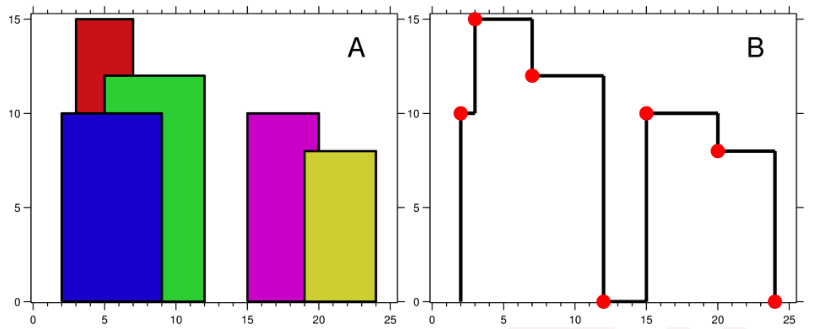
\includegraphics[width=250pt]{the-skyline-problem.png}\\
\figcaption{Skyline Problem}\label{fig:the-skyline-problem}
\end{center}

The geometric information of each building is represented by a triplet of integers [Li, Ri, Hi], where Li and Ri are the x coordinates of the left and right edge of the ith building, respectively, and Hi is its height. It is guaranteed that 0 ≤ Li, Ri ≤ INT_MAX, 0 < Hi ≤ INT_MAX, and Ri - Li > 0. You may assume all buildings are perfect rectangles grounded on an absolutely flat surface at height 0.

For instance, the dimensions of all buildings in Figure A are recorded as: [ [2 9 10], [3 7 15], [5 12 12], [15 20 10], [19 24 8] ] .

The output is a list of "key points" (red dots in Figure B) in the format of [ [x1,y1], [x2, y2], [x3, y3], ... ] that uniquely defines a skyline. A key point is the left endpoint of a horizontal line segment. Note that the last key point, where the rightmost building ends, is merely used to mark the termination of the skyline, and always has zero height. Also, the ground in between any two adjacent buildings should be considered part of the skyline contour.

For instance, the skyline in Figure B should be represented as:[ [2 10], [3 15], [7 12], [12 0], [15 10], [20 8], [24, 0] ].



Notes:

\begin{enumerate}
\item The number of buildings in any input list is guaranteed to be in the range [0, 10000].
\item The input list is already sorted in ascending order by the left x position Li.
\item The output list must be sorted by the x position.
\item There must be no consecutive horizontal lines of equal height in the output skyline. For instance, [...[2 3], [4 5], [7 5], [11 5], [12 7]...] is not acceptable; the three lines of height 5 should be merged into one in the final output as such: [...[2 3], [4 5], [12 7], ...]
\end{enumerate}

\subsubsection{分析}
Nil

\subsubsection{分治法}
\begin{Code}
// 時間複雜度O(nlogn),空間複雜度O(n)
class Solution {
public:
    vector<vector<int>> getSkyline(vector<vector<int>>& buildings) {
        return DFS(buildings, 0, buildings.size());
    }
private:
    vector<vector<int>> DFS(vector<vector<int>>& buildings, int start, int end)
    {
        if (start == end)
        {
            return vector<vector<int>>();
        }
        else if (end - start == 1)
        {
            vector<vector<int>> result;
            int& startX = buildings[start][0];
            int& startY = buildings[start][2];
            int& endX = buildings[start][1];
            result.push_back({startX, startY});
            result.push_back({endX, 0});

            return result;
        }

        int mid = start + (end - start) / 2;
        auto left = DFS(buildings, start, mid);
        auto right = DFS(buildings, mid, end);

        return mergeSkylines(left, right);
    }
    vector<vector<int>> mergeSkylines(const vector<vector<int>>& left, const vector<vector<int>>& right)
    {
        int lN = left.size();
        int rN = right.size();
        int lp, rp, curP;
        int ly, ry, curY;
        int x, maxY;
        vector<vector<int>> output; output.reserve(lN + rN);
        lp = rp = curP = 0;
        ly = ry = curY = 0;
        x = maxY = 0;

        while (lp < lN && rp < rN)
        {
            if (left[lp][0] < right[rp][0])
            {
                x = left[lp][0];
                ly = left[lp][1];
                lp++;
            }
            else
            {
                x = right[rp][0];
                ry = right[rp][1];
                rp++;
            }

            maxY = max(ly, ry);

            if (curY != maxY)
            {
                UpdateOutput(output, x, maxY);
                curY = maxY;
            }
        }

        if (lp < lN)
            AppendSkylines(output, left, lp, lN, curY);
        else
            AppendSkylines(output, right, rp, rN, curY);


        return output;
    }
    void UpdateOutput(vector<vector<int>>& output, int x, int y)
    {
        if (output.empty() || output.back()[0] != x)
            output.push_back({x, y});
        else
            output.back()[1] = y;
    }
    void AppendSkylines(vector<vector<int>>& output
                        , const vector<vector<int>>& skyline, int p, int N, int curY)
    {
        while (p < N)
        {
            const int& x = skyline[p][0];
            const int& y = skyline[p][1];
            p++;

            if (curY != y)
            {
                UpdateOutput(output, x, y);
                curY = y;
            }
        }
    }
};
\end{Code}


\section{小結} %%%%%%%%%%%%%%%%%%%%%%%%%%%%%%
\label{sec:dfs-template}


\subsection{適用場景}

\textbf{輸入數據}:如果是遞歸數據結構,如單鏈表,二叉樹,集合,則百分之百可以用深搜;如果是非遞歸數據結構,如一維數組,二維數組,字符串,圖,則概率小一些。

\textbf{狀態轉換圖}:樹或者圖。

\textbf{求解目標}:必須要走到最深(例如對於樹,必須要走到葉子節點)才能得到一個解,這種情況適合用深搜。


\subsection{思考的步驟}
\begin{enumerate}
\item 是求路徑條數,還是路徑本身(或動作序列)?深搜最常見的三個問題,求可行解的總數,求一個可行解,求所有可行解。
    \begin{enumerate}
	\item 如果是路徑條數,則不需要存儲路徑。
    \item 如果是求路徑本身,則要用一個數組\fn{path[]}存儲路徑。跟寬搜不同,寬搜雖然最終求的也是一條路徑,但是需要存儲擴展過程中的所有路徑,在沒找到答案之前所有路徑都不能放棄;而深搜,在搜索過程中始終只有一條路徑,因此用一個數組就足夠了。
    \end{enumerate}

\item 只要求一個解,還是要求所有解?如果只要求一個解,那找到一個就可以返回;如果要求所有解,找到了一個後,還要繼續擴展,直到遍歷完。廣搜一般只要求一個解,因而不需要考慮這個問題(廣搜當然也可以求所有解,這時需要擴展到所有葉子節點,相當於在內存中存儲整個狀態轉換圖,非常佔內存,因此廣搜不適合解這類問題)。

\item 如何表示狀態?即一個狀態需要存儲哪些些必要的數據,才能夠完整提供如何擴展到下一步狀態的所有信息。跟廣搜不同,深搜的慣用寫法,不是把數據記錄在狀態\fn{struct}裏,而是添加函數參數(有時為了節省遞歸堆棧,用全局變量),\fn{struct}裏的字段與函數參數一一對應。

\item 如何擴展狀態?這一步跟上一步相關。狀態裏記錄的數據不同,擴展方法就不同。對於固定不變的數據結構(一般題目直接給出,作為輸入數據),如二叉樹,圖等,擴展方法很簡單,直接往下一層走,對於隱式圖,要先在第1步裏想清楚狀態所帶的數據,想清楚了這點,那如何擴展就很簡單了。

\item 終止條件是什麼?終止條件是指到了不能擴展的末端節點。對於樹,是葉子節點,對於圖或隱式圖,是出度為0的節點。

\item {收斂條件是什麼?收斂條件是指找到了一個合法解的時刻。如果是正向深搜(父狀態處理完了才進行遞歸,即父狀態不依賴子狀態,遞歸語句一定是在最後,尾遞歸),則是指是否達到目標狀態;如果是逆向深搜(處理父狀態時需要先知道子狀態的結果,此時遞歸語句不在最後),則是指是否到達初始狀態。

由於很多時候終止條件和收斂條件是是合二為一的,因此很多人不區分這兩種條件。仔細區分這兩種條件,還是很有必要的。

為了判斷是否到了收斂條件,要在函數接口裏用一個參數記錄當前的位置(或距離目標還有多遠)。如果是求一個解,直接返回這個解;如果是求所有解,要在這裏收集解,即把第一步中表示路徑的數組\fn{path[]}複製到解集合裏。}

\item 關於判重
    \begin{enumerate}
    \item 是否需要判重?如果狀態轉換圖是一棵樹,則不需要判重,因為在遍歷過程中不可能重複;如果狀態轉換圖是一個DAG,則需要判重。這一點跟BFS不一樣,BFS的狀態轉換圖總是DAG,必須要判重。
    \item 怎樣判重?跟廣搜相同,見第 \S \ref{sec:bfs-template} 節。同時,DAG説明存在重疊子問題,此時可以用緩存加速,見第8步。
    \end{enumerate}

\item 如何加速?
    \begin{enumerate}
    \item 剪枝。深搜一定要好好考慮怎麼剪枝,成本小收益大,加幾行代碼,就能大大加速。這裏沒有通用方法,只能具體問題具體分析,要充分觀察,充分利用各種信息來剪枝,在中間節點提前返回。
    \item 緩存。
        \begin{enumerate}
            \item 前提條件:狀態轉換圖是一個DAG。DAG=>存在重疊子問題=>子問題的解會被重複利用,用緩存自然會有加速效果。如果依賴關係是樹狀的(例如樹,單鏈表等),沒必要加緩存,因為子問題只會一層層往下,用一次就再也不會用到,加了緩存也沒什麼加速效果。
            \item 具體實現:可以用數組或HashMap。維度簡單的,用數組;維度複雜的,用HashMap,C++有\fn{map},C++ 11以後有\fn{unordered_map},比\fn{map}快。
        \end{enumerate}
    
    \end{enumerate}
\end{enumerate}

拿到一個題目,當感覺它適合用深搜解決時,在心裏面把上面8個問題默默回答一遍,代碼基本上就能寫出來了。對於樹,不需要回答第5和第8個問題。如果讀者對上面的經驗總結看不懂或感覺“不實用”,很正常,因為這些經驗總結是我做了很多題目後總結出來的,從思維的發展過程看,“經驗總結”要晚於感性認識,所以這時候建議讀者先做做前面的題目,積累一定的感性認識後,再回過頭來看這一節的總結,一定會有共鳴。


\subsection{代碼模板}

\begin{Codex}[label=dfs_template.cpp]
/**
 * dfs模板.
 * @param[in] input 輸入數據指針
 * @param[out] path 當前路徑,也是中間結果
 * @param[out] result 存放最終結果
 * @param[inout] cur or gap 標記當前位置或距離目標的距離
 * @return 路徑長度,如果是求路徑本身,則不需要返回長度
 */
void dfs(type &input, type &path, type &result, int cur or gap) {
    if (數據非法) return 0;   // 終止條件
    if (cur == input.size()) { // 收斂條件
    // if (gap == 0) {
        將path放入result
    }

    if (可以剪枝) return;

    for(...) { // 執行所有可能的擴展動作
        執行動作,修改path
        dfs(input, step + 1 or gap--, result);
        恢復path
    }
}
\end{Codex}


\subsection{深搜與回溯法的區別}
深搜(Depth-first search, DFS)的定義見\myurl{http://en.wikipedia.org/wiki/Depth_first_search},回溯法(backtracking)的定義見\myurl{http://en.wikipedia.org/wiki/Backtracking}

\textbf{回溯法 = 深搜 + 剪枝}。一般大家用深搜時,或多或少會剪枝,因此深搜與回溯法沒有什麼不同,可以在它們之間畫上一個等號。本書同時使用深搜和回溯法兩個術語,但讀者可以認為二者等價。

深搜一般用遞歸(recursion)來實現,這樣比較簡潔。

深搜能夠在候選答案生成到一半時,就進行判斷,拋棄不滿足要求的答案,所以深搜比暴力搜索法要快。


\subsection{深搜與遞歸的區別}
\label{sec:dfs-vs-recursion}

深搜經常用遞歸(recursion)來實現,二者常常同時出現,導致很多人誤以為他倆是一個東西。

深搜,是邏輯意義上的算法,遞歸,是一種物理意義上的實現,它和迭代(iteration)是對應的。深搜,可以用遞歸來實現,也可以用棧來實現;而遞歸,一般總是用來實現深搜。可以説,\textbf{遞歸一定是深搜,深搜不一定用遞歸}。

遞歸有兩種加速策略,一種是\textbf{剪枝(prunning)},對中間結果進行判斷,提前返回;一種是\textbf{緩存},緩存中間結果,防止重複計算,用空間換時間。

其實,遞歸+緩存,就是 memoization。所謂\textbf{memoization}(翻譯為備忘錄法,見第 \S \ref{sec:dp-vs-memoization}節),就是"top-down with cache"(自頂向下+緩存),它是Donald Michie 在1968年創造的術語,表示一種優化技術,在top-down 形式的程序中,使用緩存來避免重複計算,從而達到加速的目的。

\textbf{memoization 不一定用遞歸},就像深搜不一定用遞歸一樣,可以在迭代(iterative)中使用 memoization 。\textbf{遞歸也不一定用 memoization},可以用memoization來加速,但不是必須的。只有當遞歸使用了緩存,它才是 memoization 。

既然遞歸一定是深搜,為什麼很多書籍都同時使用這兩個術語呢?在遞歸味道更濃的地方,一般用遞歸這個術語,在深搜更濃的場景下,用深搜這個術語,讀者心裏要弄清楚他倆大部分時候是一回事。在單鏈表、二叉樹等遞歸數據結構上,遞歸的味道更濃,這時用遞歸這個術語;在圖、隱式圖等數據結構上,深搜的味道更濃,這時用深搜這個術語。
